% PREÁMBULO -------------------------------------
  
% Definir la clase de documento
\documentclass[a4paper, 11pt]{article}

% Codificación de entrada
\usepackage[utf8]{inputenc}

% Idioma
\usepackage[spanish]{babel}

% Geometría
\usepackage[left = 2cm, right = 2.5cm, top = 3cm, bottom = 2.2cm]{geometry}

% Inserción de figuras
\usepackage{graphicx}

\usepackage{subcaption}
%\usepackage{subfigure} % Revisar el error que esta generando

% Hipervínculos
\usepackage{hyperref}

\usepackage{titlesec}

% Matemáticas
\usepackage{amsfonts}
\usepackage{amsmath}
\usepackage{amssymb}
\usepackage{amsthm}
\newtheorem{defi}{Definición}[section]
\newtheorem{lema}{Lema}[section]
\newtheorem{teo}{Teorema}[section]
\newtheorem{coro}{Corolario}[section]


\usepackage{float}

% Crear párrafos
\usepackage{lipsum}

% Multicolumnas
\usepackage{multicol}


% Espacios en párrafos
\usepackage{setspace}




%Colores
\usepackage{xcolor}
\definecolor{gris}{gray}{0.9}
\definecolor{azul}{rgb}{0.0, 0.48, 0.65}

% Información del documento
\author{Manuel Merino Huaman}
\title{Modo matemático en \LaTeX}
\date{26 de febrero de 2023}

% Configuraciones en los listados de texto - Numerados
%% Nivel 1
\renewcommand{\theenumi}{\arabic{enumi}}
\renewcommand{\labelenumi}{\arabic{enumi}.}

%% Nivel 2
\renewcommand{\theenumii}{\alph{enumii}}
\renewcommand{\labelenumii}{\arabic{enumii}.$\alph{enumii}$}

%% Nivel 3
\renewcommand{\theenumiii}{\roman{enumiii}}
\renewcommand{\labelenumiii}{\roman{enumiii})}

%% Nivel 4
\renewcommand{\theenumiv}{\alph{enumiv}}
\renewcommand{\labelenumiv}{\alph{enumiv}.}

% Configuraciones en los listados de texto - No numerados
%% Nivel 1
\renewcommand{\labelitemi}{$\checkmark$}

%% Nivel 2
\renewcommand{\labelitemii}{$\bigstar$}

%% Nivel 3
\renewcommand{\labelitemiii}{$\dagger$}

%% Nivel 4
\renewcommand{\labelitemiv}{$\circledast$}

% Creación de comandos
%% Números naturales
\newcommand{\N}{\mathbb{N}}
%% Números enteros
\newcommand{\Z}{\mathbb{Z}}
%% Números racionales
\newcommand{\Q}{\mathbb{Q}}
%% Números irracionales
\newcommand{\I}{\mathbb{I}}
%% Números reales
\newcommand{\R}{\mathbb{R}}
%% Números complejos
\newcommand{\C}{\mathbb{C}}

% Crear funciones trigonométricas inversas
\newcommand{\arccot}{\text{arccot}}
\newcommand{\arcsec}{\text{arcsec}}
\newcommand{\arccsc}{\text{arccsc}}


\usepackage{rotating}
\usepackage{tabularx} % Permite hacer cambios en el contenido de una tabla
\usepackage{multirow}

\usepackage{caption}
\captionsetup[table]{
   name = Tabla,
   labelsep = newline,
   justification = raggedright,
   singlelinecheck = false,
   labelfont = bf
}

    
% Máximo entero
\usepackage{mathabx}



% Entorno del documento
\begin{document}

    \maketitle

    % Section
    \section{Tablas}
    
    % Table 1
    \begin{table}[h]
        \raggedright
        \caption{Título de la tabla}
          \begin{tabular}{|l|l|c|l|r|}
             \hline
             Nombres & Apellidos & Edad & País & Puntaje  \\
             \hline
             Manuel & Merino Huaman& 28& Perú& 89.76\\
             Pablo & Perez Zarumilla& 31& Colomabia & 76.4\\
             Estrella & Contreras Montalvo & 27 & Perú & 90.3 \\
             Cristian & Castro Villareal& 20& Chile & 90.214 \\
            \hline
           \end{tabular}
         \vspace{2mm}
        \caption*{\it Nota: Creación propia.}  
        \label{tab: tabla prueba}
    \end{table}
    
    % Table 2
    \begin{table}[!hbt]
        \raggedright
        \caption{Lista de resultados del Examen Final 2021}
            \begin{tabular}{|l|c|c|c|}
                \hline
                 Nombre  & \begin{sideways} Matemáticas \, \end{sideways}& \begin{sideways} Física \end{sideways}   &  \begin{sideways} Química \end{sideways}     \\
                \hline
                 Manuel & 97 & 90 & 87 \\
                \hline 
                 Cristian & 90 & 70 & 56 \\
                \hline
                 Martin &  80 & 98  & 91 \\
                \hline
            \end{tabular}
            
        \vspace{2mm}
        \caption*{\it Nota: Creación propia.}
        \label{tab: tabular-5}
    \end{table}
   
    % Table 3
    \begin{table}[h]
        \centering
        \begin{tabular}{|l|l|r|m{9.25cm}|} % usando tabularx (p{} o m{} o b{})
            \hline
            Game title &  Gabinete & Índice & Observación\\
            \hline
            Ocean Magic &  Crystal Dual  & 1.78  & Ha sido un juego de buen rendimiento para la región. \\ 
            \hline
            Scarab & Crystal Slant  &  2.45 & El mejor de colombia.   \\ 
            \hline
            Olimpus & Peak Slant & 3.21 & Multijuego con los mejores resultados en la región de Latinoamérica. Ocurrió algunos problemas con los pozos en el primer trimestre.\\
            \hline 
        \end{tabular}
        \caption{Tabla N°3}
        \label{tab:my_label 1}
    \end{table}

    % Table 4
    \begin{table}[H] % Note: Manuel no recomienda usar el "H" en book 
        \centering
        \begin{tabular}{|c|c|c|c|c|c|}
         \hline 
         \multirow{2}{*}{Nombres} &  \multicolumn{4}{c|}{Cursos} & \multirow{2}{*}{Total}\\
         \cline{2-5}
                 & Mate & Fis & Quim & Inglés &     \\
         \hline 
         Manuel & 95 & 89 & 82 & 72 & 338\\
         \hline 
         Melissa & 80 & 75 & 85 & 50 & 290 \\
         \hline 
         Moises & 60 & 50 & 40 & 60 & 210 \\
         \hline 
         Martin & 85 & 98 & 95 & 90 & 368 \\
         \hline 
        \end{tabular}
        \caption{Tabla N°4}
        \label{tab:my_label 2}
    \end{table}


    % Section 
    \section{Figuras}

        % figure 1
        \begin{figure}[ht]
            \centering
            \caption{Mi primera inserción de figura en \LaTeX}
            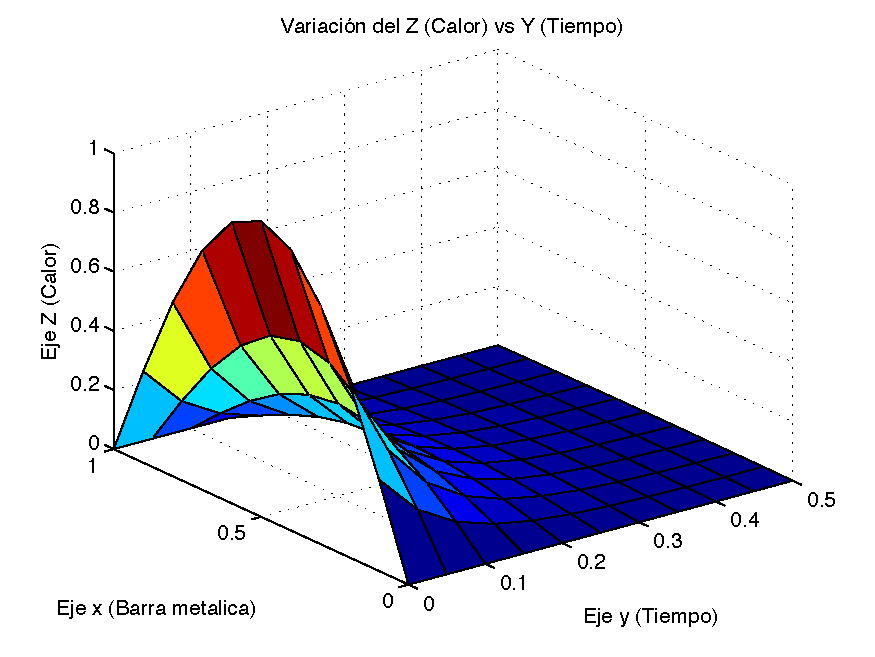
\includegraphics[width = 10cm, height = 6cm]{04_ENTORNOS_FLOTANTES/images/Grafica3D.pdf}
            \label{fig: Grafica 3D - 1}
        \end{figure}
        
        % figure 2
        \begin{figure}[ht]
            \centering
            \caption{Mi primera inserción de figura en \LaTeX}
            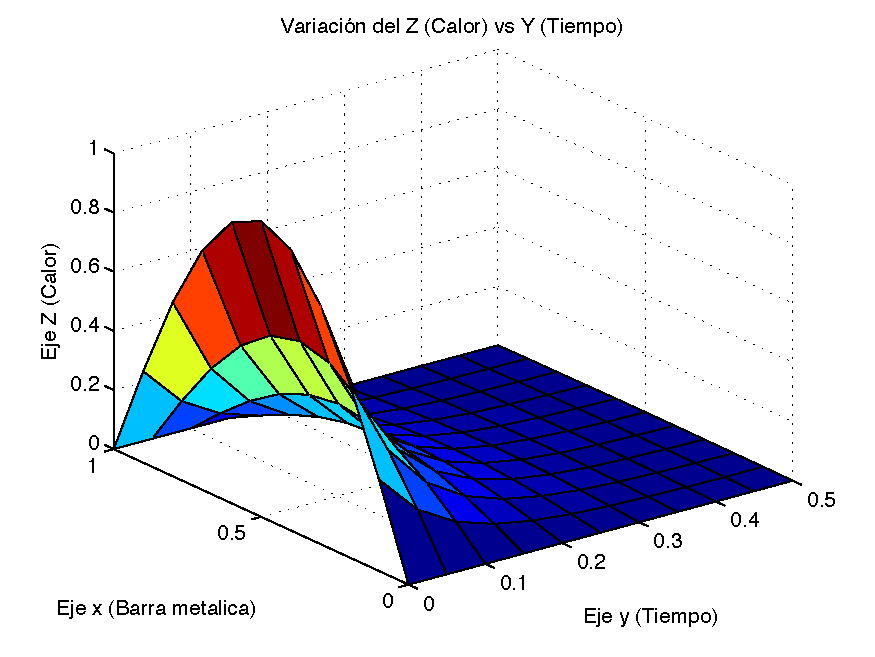
\includegraphics[width = \linewidth]{04_ENTORNOS_FLOTANTES/images/Grafica3D.pdf}
            \label{fig: Grafica3D - 2}
        \end{figure}

        % figure 3
        \begin{figure}[ht]
            \centering
            \caption{Mi primera inserción de figura en \LaTeX}
            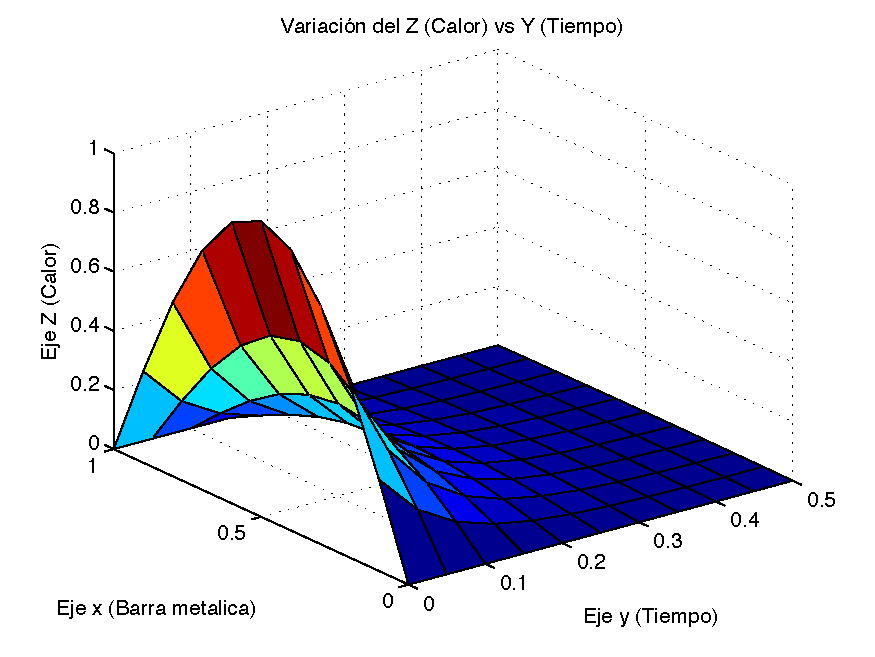
\includegraphics[width = 0.7\linewidth]{04_ENTORNOS_FLOTANTES/images/Grafica3D.pdf}
            \label{fig: Grafica3D - 3}
        \end{figure}

        % figure 4
        \begin{figure}[ht]
            \centering
            \caption{Mi primera inserción de figura en \LaTeX}
            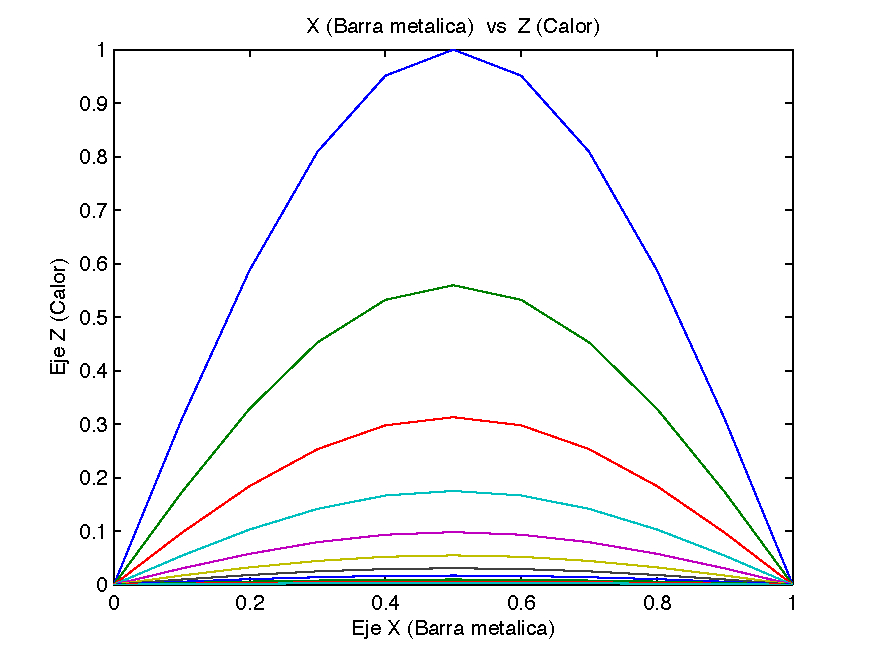
\includegraphics[scale = 1]{04_ENTORNOS_FLOTANTES/images/Grafica2D.pdf}
            \label{fig: Grafica2D - 1}
        \end{figure}

        % figure 5
        \begin{figure}[ht]
            \centering
            \caption{Mi primera inserción de figura en \LaTeX}
            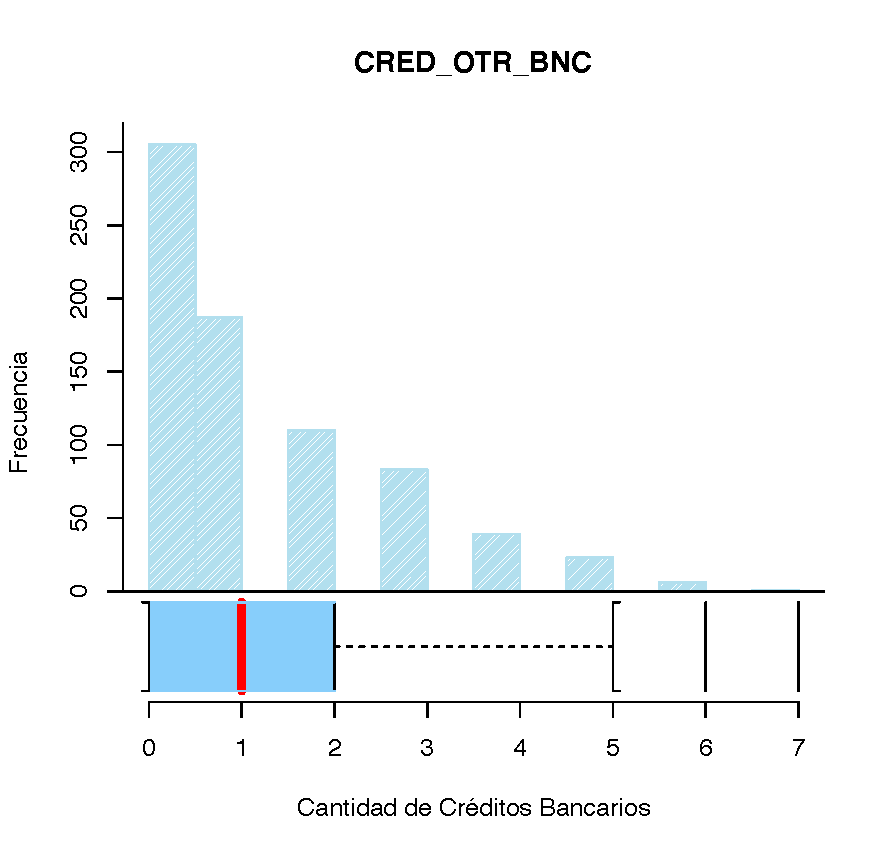
\includegraphics[scale = 1]{04_ENTORNOS_FLOTANTES/images/mifigura.pdf}
            \label{fig: minifigura.pdf}
        \end{figure}
        
        % figure 6
        \begin{figure}[ht]
            \centering
            \caption{Mi primera inserción de figura en \LaTeX}
            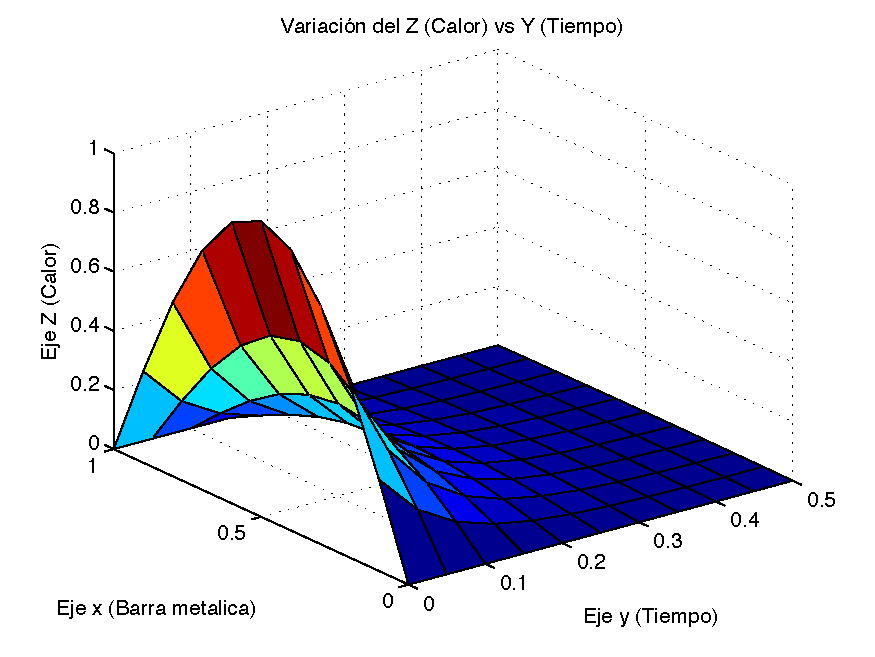
\includegraphics[width = 0.7\linewidth, clip = true, trim = 1.5cm 1cm 0cm 1cm]{04_ENTORNOS_FLOTANTES/images/Grafica3D.pdf}
            \label{fig: Graficaaa}
        \end{figure}






%%%%%%% Revisar okkkkkkkkkkkkkkkkkkkkkkkkkkkkkkk
        %\begin{figure}[h]
        %    \centering
        %    \subfigure[Imagen en R]{
        %    \subcaption[width = 0.3\linewidth]{04_ENTORNOS_FLOTANTES/images/mifigura.pdf}
        %    }
        %    \caption{Ejemplo de sub-figura en horizontal}
        %    \label{fig: subfiguras horizontal}
        %\end{figure}
        
        % figure 7
        \begin{figure}[ht]
            \centering
            \begin{subfigure}[b]{0.49\textwidth}
                \centering
                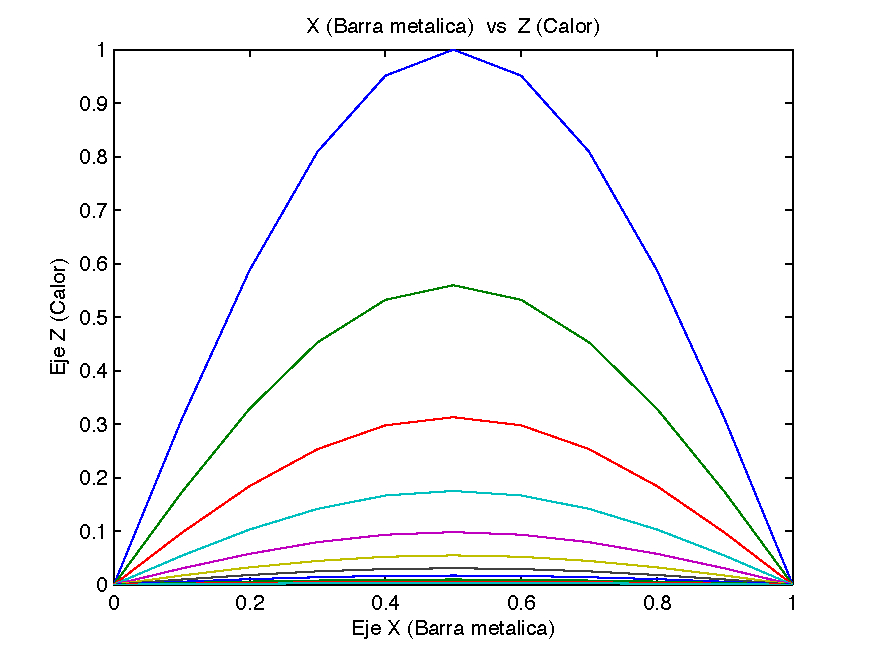
\includegraphics[width = \textwidth]{04_ENTORNOS_FLOTANTES/images/Grafica2D.pdf}
                \caption{Minifigura - ejemplo}
                \label{fig: Minifigura - ejemplo}
            \end{subfigure}
            \hfill 
            \begin{subfigure}[b]{0.49\textwidth}
                \centering
                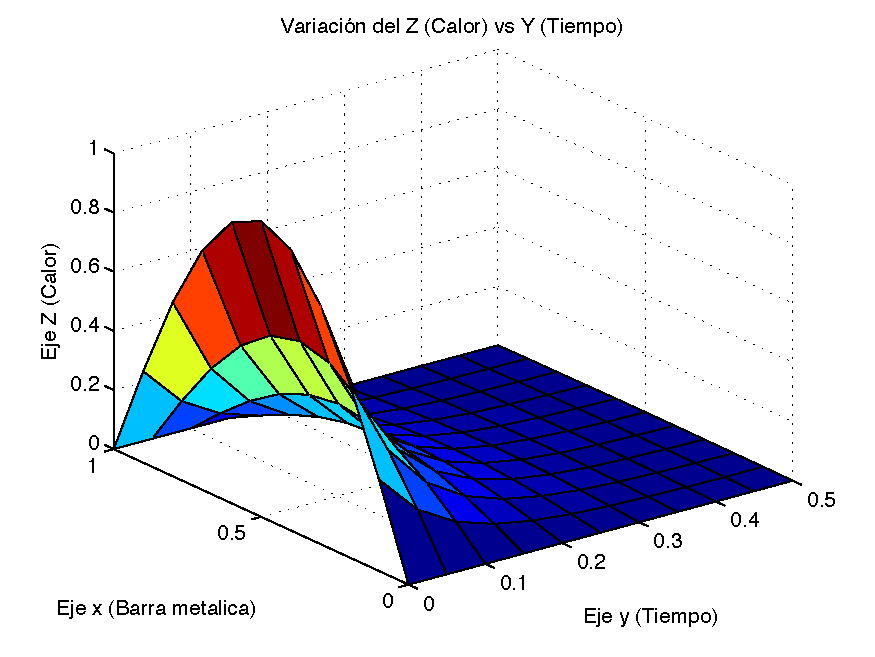
\includegraphics[width = \textwidth]{04_ENTORNOS_FLOTANTES/images/Grafica3D.pdf}
                \caption{Gráfica en 2D - ejemplo}
                \label{fig: Gráfica en 2D - ejemplo}
            \end{subfigure}
                \caption{Ejemplo de subfiguras}
                \label{fig: Ejemplo de subfiguras}
        \end{figure}


        % figure 8
        \begin{figure}[ht]
            \centering
            \begin{subfigure}[b]{0.3\textwidth}
                \centering
                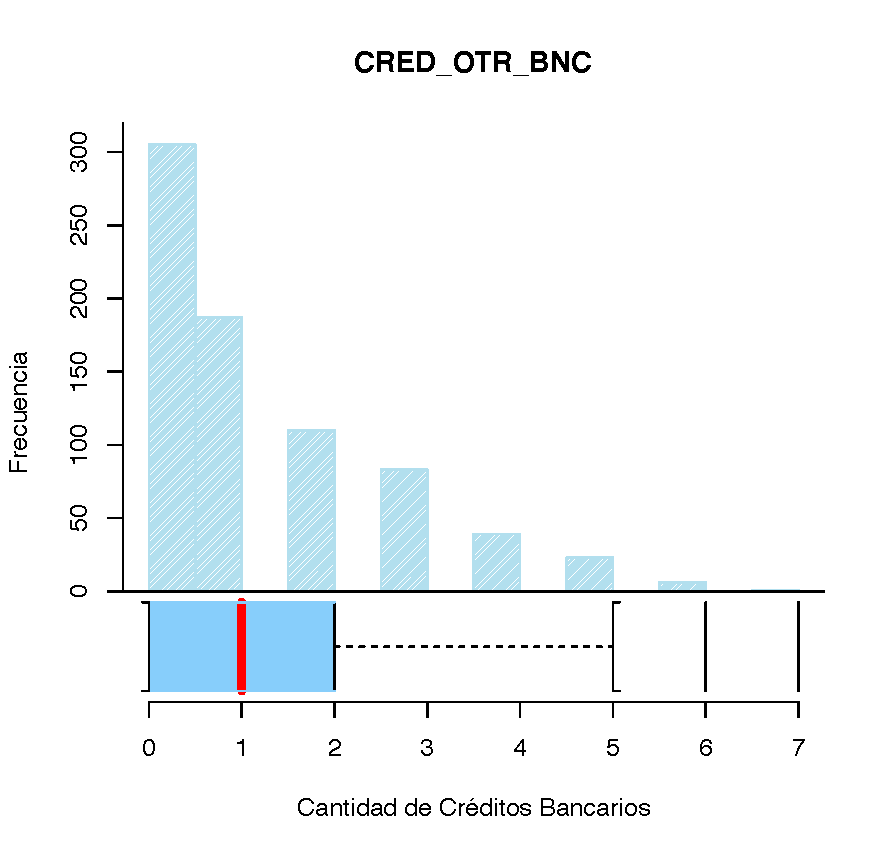
\includegraphics[width=\textwidth]{04_ENTORNOS_FLOTANTES/images/mifigura.pdf}
                \caption{Minifigura}
                \label{fig: minifigura}
            \end{subfigure}
            \hfill 
            \begin{subfigure}[b]{0.3\textwidth}
                \centering
                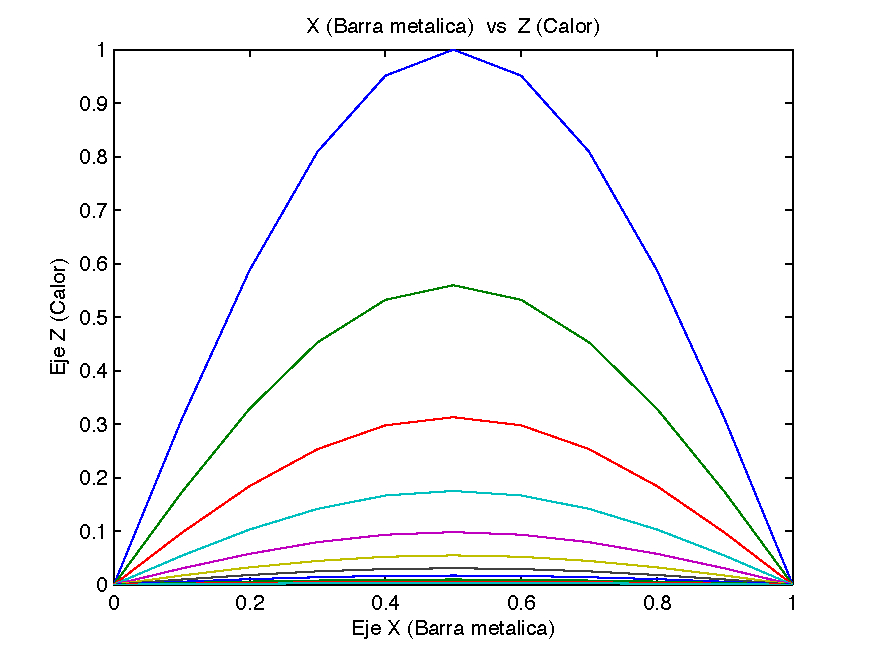
\includegraphics[width=\textwidth]{04_ENTORNOS_FLOTANTES/images/Grafica2D.pdf}
                \caption{Gráfica en 2D}
                \label{fig: Gráfica en 2D}
            \end{subfigure}
            \hfill
            \begin{subfigure}[b]{0.3\textwidth}
                \centering
                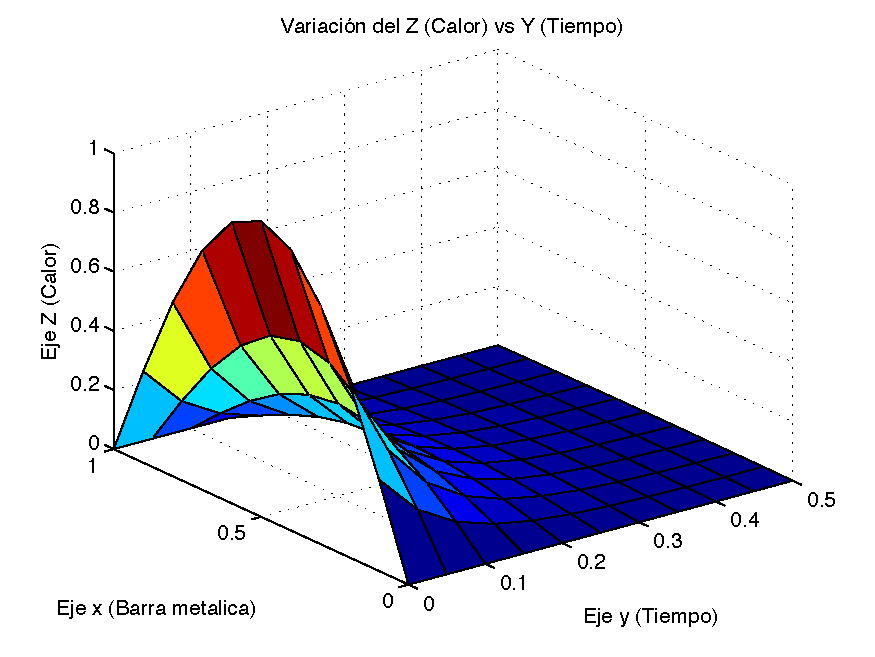
\includegraphics[width=\textwidth]{04_ENTORNOS_FLOTANTES/images/Grafica3D.pdf}
                \caption{Gráfica en 3D}
                \label{fig: Gráfica en 3D}
            \end{subfigure}
            \caption{Tres gráficas simples}
            \label{fig: tres gráficas simples}
        \end{figure}
        
%%%%%%% Revisar
        
        

        


        

    
\end{document}